%\begin{itemize}
%    \item Initial findings on feature importance and model reasoning using XAI techniques for hierarchical models.
%    \item Observations on model performance and key features at different levels.
%\end{itemize}


\section{Preliminary Results}\label{sec:preliminary_results}

The preliminary results focus mainly on the practical application of SHAP values in hierarchical forecasting models
rather than on the theoretical aspects of feature importance.
As preliminary results, we present mean average SHAP values at different aggregation levels.
These provide an overview of the main contributors to the forecast at different levels of the hierarchy.

Furthermore, we visualise the distribution of SHAP values at different aggregation levels using violin plots,
which provide a representation of variability and density of SHAP values for each feature across the hierarchy.
This double representation allows for a more detailed analysis of the contribution of features to the forecast, for example,
if a feature contributes positively or negatively to the forecast.
In the following, we present several cases of different aggregation levels, starting from the global level to the store and product level,
but it is not meant to be exhaustive.

%\subsection{Global SHAP values} \label{subsec:global_shap}

At the global level, the SHAP values\ref{fig:global_shap} show that the most important features are the lagged sales values, especially the sales value of lag 1, which has the highest SHAP value.
This is expected as prior sales are the most important factor in predicting future sales.
The violin plot in Figure \ref{fig:global_shap_violin} shows the distribution of SHAP values for each feature.
It shows that the actual impact of the lag value is most of the time negative,
as after a week with higher sales, demand the following week can drop.

\begin{figure}[h]
    \centering
    \begin{minipage}{.45\textwidth}
        \centering
        \begin{subfigure}{\textwidth}
            \centering
            \includegraphics[width=\linewidth]{sections/img/shap_global}
            \caption{Global SHAP values}
            \label{fig:global_shap}
        \end{subfigure}%
%        \vskip\baselineskip
        \begin{subfigure}{\textwidth}
            \centering
            \includegraphics[width=\linewidth]{sections/img/shap_global_vioalin}
            \caption{Global SHAP violin plot}
            \label{fig:global_shap_violin}
        \end{subfigure}%
    \end{minipage}%
    \hfill
    \begin{minipage}{.45\textwidth}
        \centering
        % Add any additional subfigures here if needed
    \end{minipage}
    \caption{Global summary}\label{fig:global_summary}
\end{figure}


%%%%%%%%%%%%%%%%%%%%%%%%%%%%%%%%

%\subsection{State level SHAP values} \label{subsec:state_shap}
In case of state-level grouping, the number of samples differs for the two groups,
one of them having only two stores included.
This can be observed in the wider distribution on the violin plot of the Texas(TX) state.

\begin{figure}
    \centering
    \begin{minipage}{.45\textwidth}
        \centering
        \begin{subfigure}{\textwidth}
            \centering
            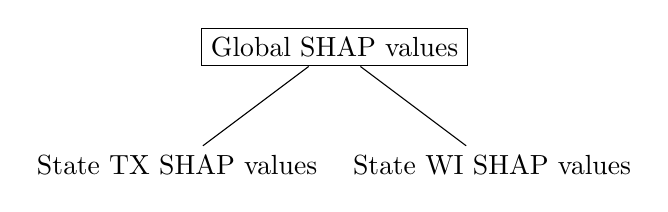
\begin{tikzpicture}
            [level 1/.style={sibling distance=40mm},
                level 2/.style={sibling distance=15mm}]
                \node[rectangle,draw] {Global SHAP values}
                child {node {State TX SHAP values} }
                child {node {State WI SHAP values}};
            \end{tikzpicture}
            \caption{State level SHAP values}
        \end{subfigure}%
        \vskip\baselineskip
        \begin{subfigure}{\textwidth}
            \centering
            \includegraphics[width=\linewidth]{sections/img/state_product}
            \caption{State level SHAP values}
            \label{fig:sub2}
        \end{subfigure}%
    \end{minipage}%
    \hfill
    \begin{minipage}{.45\textwidth}
        \centering
        \begin{subfigure}{\textwidth}
            \centering
            \includegraphics[width=\linewidth]{sections/img/state_tx_violin}
            \caption{TX state product SHAP summary}
            \label{fig:state_tx_violin_sub3}
        \end{subfigure}%
        \vskip\baselineskip
        \begin{subfigure}{\textwidth}
            \centering
            \includegraphics[width=\linewidth]{sections/img/state_wi_violin}
            \caption{WI state product SHAP summary}
            \label{fig:State_wi_violin_sub4}
        \end{subfigure}
    \end{minipage}
\end{figure}
%############################################################

%\subsection{State and product grouping}\label{subsec:state_prod_shap}
% TODO: The first lag value almost every time positively affects the forecast
\begin{figure}
    \centering
    \begin{minipage}{.45\textwidth}
        \centering
        \begin{subfigure}{\textwidth}
            \centering
            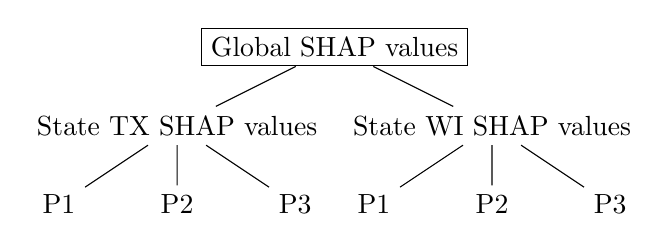
\begin{tikzpicture}
            [level 1/.style={sibling distance=40mm, level distance=10mm},
                level 2/.style={sibling distance=15mm, level distance=10mm}]
                \node[rectangle,draw] {Global SHAP values}
                child {node {State TX SHAP values}
                child {node {P1}}
                child {node {P2}}
                child {node {P3}}
                }
                child {node {State WI SHAP values}
                child {node {P1}}
                child {node {P2}}
                child {node {P3}}
                };
            \end{tikzpicture}
            \caption{Aggregation levels}
        \end{subfigure}%
        \vskip\baselineskip
        \begin{subfigure}{\textwidth}
            \centering
            \includegraphics[width=\linewidth]{sections/img/bar_state_product}
            \caption{State and product level SHAP values}
            \label{fig:state_product_sub2}
        \end{subfigure}%
    \end{minipage}%
    \hfill
    \begin{minipage}{.45\textwidth}
        \centering
        \begin{subfigure}{\textwidth}
            \centering
            \includegraphics[width=\linewidth]{sections/img/state_product_violin_1}
            \caption{TX state FOODS\_3\_586 product SHAP summary}
            \label{fig:state_prod_sub3}
        \end{subfigure}%
        \vskip\baselineskip
        \begin{subfigure}{\textwidth}
            \centering
            \includegraphics[width=\linewidth]{sections/img/state_product_violin2}
            \caption{WI state FOODS\_3\_080 product SHAP summary}
            \label{fig:state_prod_violin_sub4}
        \end{subfigure}
    \end{minipage}
    \caption{State and product level summary}
\end{figure}
%\begin{figure}
%    \centering
%%    \begin{tabular}{ c c }
%    \begin{subfigure}{.5\textwidth}
%        \centering
%        \begin{tikzpicture}
%        [level 1/.style={sibling distance=40mm, level distance=10mm},
%            level 2/.style={sibling distance=15mm, level distance=10mm}]
%            \node[rectangle,draw] {Global SHAP values}
%            child {node {State TX SHAP values}
%            child {node {P1}}
%            child {node {P2}}
%            child {node {P3}}
%            }
%            child {node {State WI SHAP values}
%            child {node {P1}}
%            child {node {P2}}
%            child {node {P3}}
%            };
%        \end{tikzpicture}
%        \caption{Aggregation levels}
%    \end{subfigure}%
%%    \vskip   \baselineskip
%    \begin{subfigure}{.5\textwidth}
%        \centering
%        \includegraphics[width=\linewidth]{sections/img/bar_state_product}
%        \caption{State and product level SHAP values}
%        \label{fig:state_product_sub2}
%    \end{subfigure}%
%    \hskip  % \baselineskip
%    \begin{subfigure}{.5\textwidth}
%        \centering
%        \includegraphics[width=\linewidth]{sections/img/state_product_violin_1}
%        \caption{TX state FOODS\_3\_586 product SHAP summary}
%        \label{fig:state_prod_sub3}
%    \end{subfigure}  %
%    \begin{subfigure}{.5\textwidth}
%        \centering
%        \includegraphics[width=\linewidth]{sections/img/state_product_violin2}
%        \caption{WI state FOODS\_3\_080 product SHAP summary}
%        \label{fig:state_prod_violin_sub4}
%    \end{subfigure}
%    \caption{State and product level summary}
%%    \end{tabular}
%\end{figure}



%%%%%%%%%%%%%%%%%%%%%%%%%%%%%%%%%%%%%%%%%%%%%%%%%%%%%%%%%%%%

% Store and product level
On the lowest level of the hierarchy presented in Figure \ref{fig:store_product_summary},
deviations can be revealed in the order of importance of the features.
For example, in Figure \ref{fig:store_prod_violin_sub4e} the week-of-year feature has a greater impact
on the forecast than some of the lag values that occurred in other cases in Figure \ref{fig:store_prod_sub3}.
This can be due to the fact that the store TX\_2 has a different seasonality pattern or
might have recurring special events, since the number of events is also a feature with higher impact on this store.
What is problematic in this case is that, due to the large number of series,
representation of the mean absolute SHAP value is hardly comprehensible in the previous form of the bar plot.
As a workaround, the grouping of feature contribution of each group is presented in Figure \ref{fig:store_product_sub2}.
What can be misleading in this case is the lack of order by impact and a different scale of the $x$ axis for each feature.

\begin{figure}
    \centering
    \begin{subfigure}{\textwidth}
        \centering
        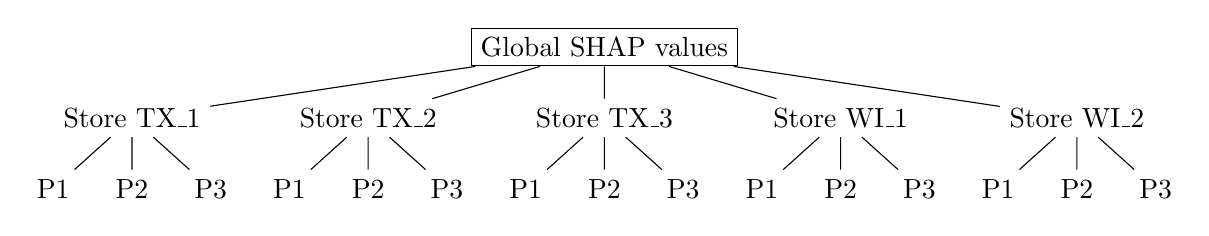
\begin{tikzpicture}
        [level 1/.style={sibling distance=30mm, level distance=9mm},
            level 2/.style={sibling distance=10mm,  level distance=9mm},]
%            level 3/.style={sibling distance=10mm}]
            \node[rectangle,draw] {Global SHAP values}
%            child {node {State TX}
            child {node {Store TX\_1}
            child {node {P1}}
            child {node {P2}}
            child {node {P3}}
            }
            child {node {Store TX\_2}
            child {node {P1}}
            child {node {P2}}
            child {node {P3}}
            }
            child {node {Store TX\_3}
            child {node {P1}}
            child {node {P2}}
            child {node {P3}}
            }
%            }
%            child {node {State WI}
            child {node {Store WI\_1}
            child {node {P1}}
            child {node {P2}}
            child {node {P3}}
            }
            child {node {Store WI\_2}
            child {node {P1}}
            child {node {P2}}
            child {node {P3}}
            };
        \end{tikzpicture}
        \caption{Aggregation levels}
    \end{subfigure}%
    \vskip\baselineskip
    \begin{subfigure}{.9\linewidth}
        \centering
     %  \includegraphics[width=0.8\linewidth, trim={0 67cm 30cm 0},clip ]{sections/img/store_product_shap2}
      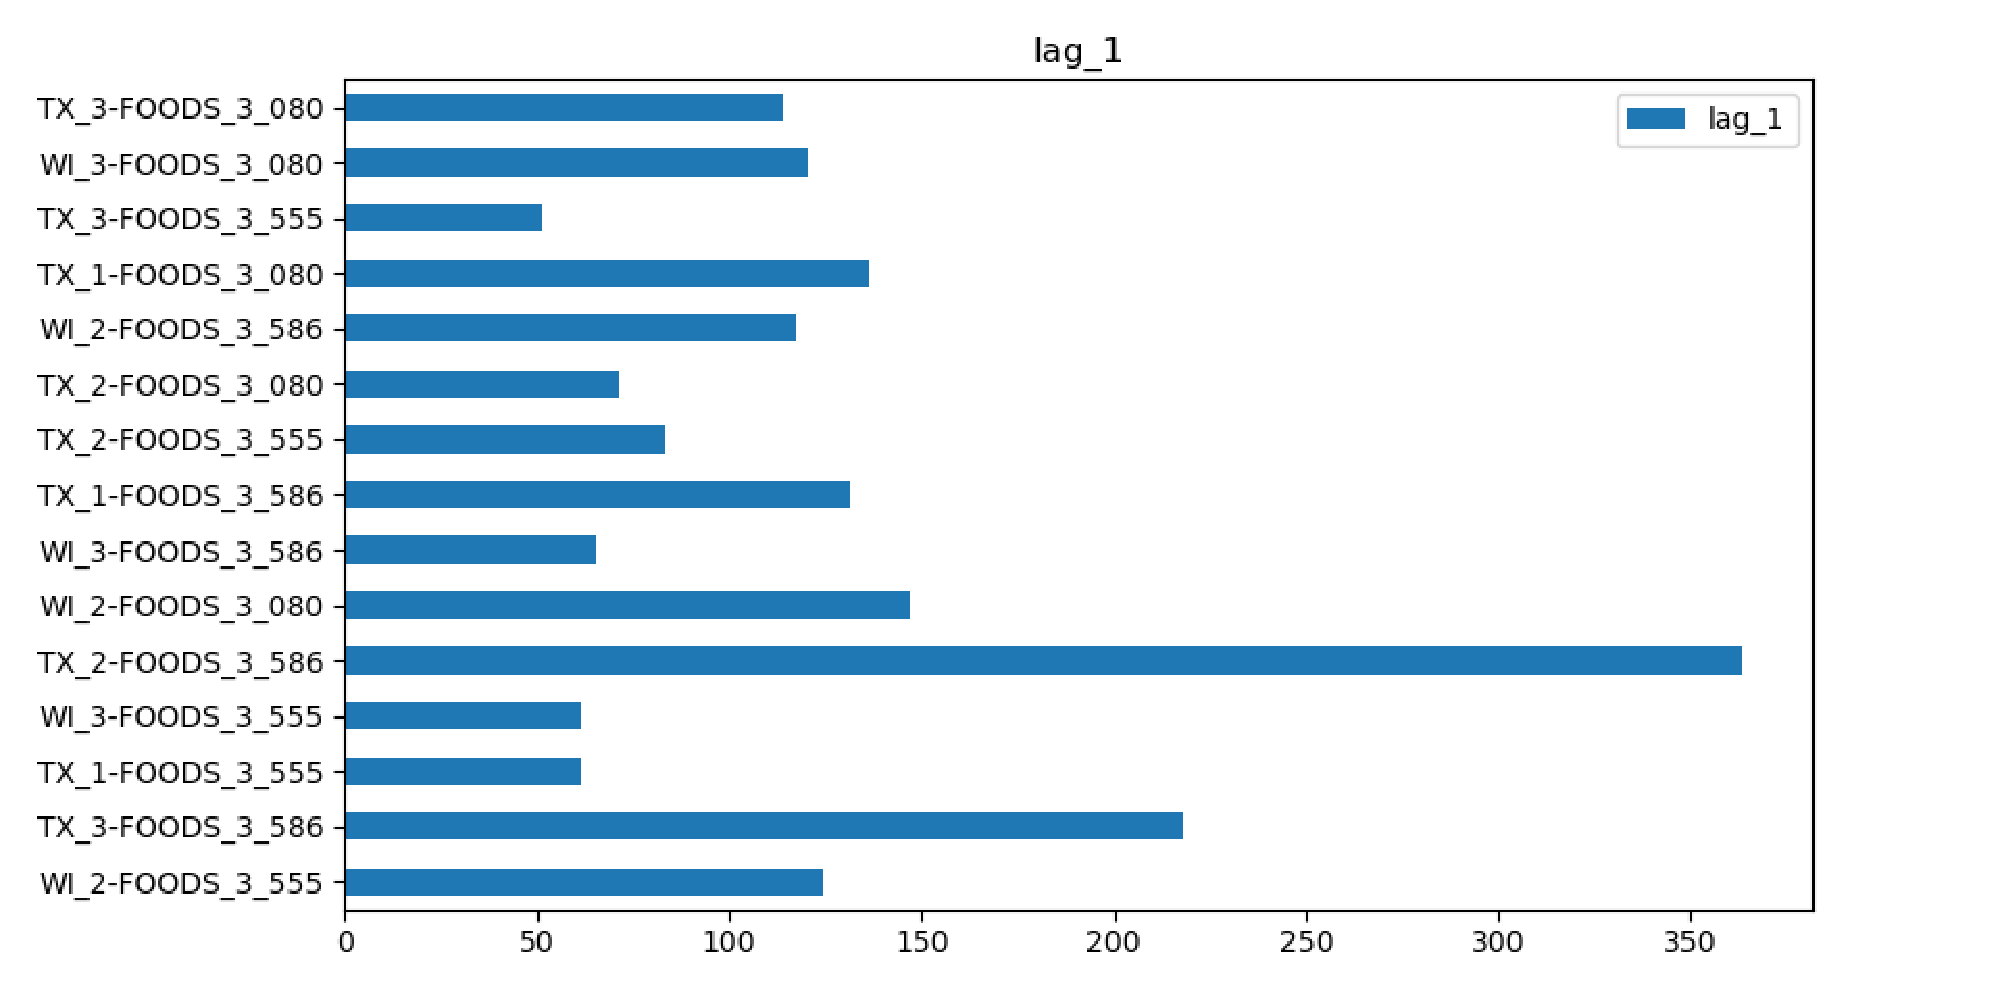
\includegraphics[width=0.8\linewidth]{sections/img/store_product_shap_2.eps}
        \caption{Store and product level SHAP values for one feature}
        \label{fig:store_product_sub2}
    \end{subfigure}%
    \vskip\baselineskip
    \begin{subfigure}{.5\textwidth}
        \centering
        \includegraphics[width=\linewidth,]{sections/img/store_product_violin3}
        \caption{Store TX\_3 FOODS\_3\_586 product SHAP summary}
        \label{fig:store_prod_sub3}
    \end{subfigure}%
    \begin{subfigure}{.5\textwidth}
        \centering
        \includegraphics[width=\linewidth]{sections/img/store_productviolin2}
        \caption{Store TX\_2 FOODS\_3\_080 product SHAP summary}
        \label{fig:store_prod_violin_sub4e}
    \end{subfigure}
    \caption{Store and product level summary}\label{fig:store_product_summary}
\end{figure}

